% Chapter 4

\chapter{Model Free Reinforcement Learning} % Main chapter title

\label{Chapter4} % For referencing the chapter elsewhere, use \ref{Chapter1} 

\section{Deep Reinforcement Learning}
\subsection{Deep Q Network}

As we so in chapter \ref{Chapter3}, to solve an unknown MDP, we use the Bellman equation \ref{bellman-equation-for-q}.
We want to approximate the function of the optimal value iteratively until the algorithms converge, but to do this, we need to maintain the experience gained in the previous iterations.
Originally, all the temporary q-value estimates were stored in a tabular, but this kind of solution worked well only with toy problems.
The solution was the use of a function approximator instead of tabular methods.
Initially, they tried whit a linear function approximation, but also that solution is not able to scale.
The first, scalable and successfully, use of neural networks as a function approximator of Q-value was introduced in 2015 by Deepmind \cite{mnih2015human}.
The solution proposed in this work is to build a Q-network and train it by adjusting the parameters $ \theta $ to reduce the mean-squared error in the Bellman equation.

This network, called \textbf{Q-Network}, takes an observation as input and then give in output, with a single forward pass, the predicted Q-values for all possible actions.

Before this solution, the use of neural networks in the framework of reinforcement learning was known to be an unstable method.
This instability has several causes: the correlation between transactions, the change in the distribution of data caused by the change in policy.
To address these problems, they introduce two variants of the q-learning algorithm. 

An \textbf{Experience Buffer Replay} was introduced to remove correlations in the observation sequence and smooth over changes in the data distribution.

So, at each time step $t$, the agent store its experience $e_t=(s_t,a_t,r_t,s_{t+1})$ in a dataset $D_t={e_1, ... ,e_t}$.
At the learning time it the agent draw a random batch of experiences from the dataset and apply a Q-learning update.  

The second variant is the use a second neural network called \textbf{Target Network} to perform a target estimate in the Q-update.
So the Q-network is trained to reach the target network predictions that use an old set of weight.
So, every C updates the Q-networks weights are cloned to generate a better set of weights for the Target-networks.
This solution makes divergence or oscillations much more unlikely.

This algorithm was tested on a set of environments that replicated the games from an old console called atari Atari 2600.
Reinforcement learning was usually applied to domains in which useful features were being crafted in low-dimensional state space.
The DQN instead, was trained directly from high-dimensional inputs that were the raw frames of the games. 

This choice led to a problem, one single frame does not contain enough information to be an effective state of an MDP since it violates the Markov property.
In fact, having one single frame is not enough to
predict the next one (for example, you cannot guess the position of an object in the next frame if you do not know its speed and direction).
So, in that case, the environment is not an MDP but is a POMDP.
To give to the network enough information they stacked more frames into one single input.

Using the frames as input allow the algorithm to be more general.
In fact, DQN was able to achieve human-level performance over 49 different games using the same network architecture and hyperparameters.

\begin{algorithm}
	\caption{Deep Q-learning with Experience Replay}
	\label{algo:DQN}
	\begin{algorithmic}[]
		\State initialize replay memory \textit{D} to capacity {N}
		\State initialize action-value function \textit{Q} with random weights {$\theta$}
        \State initialize target action-value function ${\hat{Q}}$ with weights ${\theta^-}={\theta}$
		 \For{episode=1,M}
			\State Inizialize sequence $s_1$=$x_1$ and preprocessed sequence $\phi_1= \phi(s_1)$
            \For{$t = 1,T$}
            		\State With probability $\epsilon$ select a random action $a_t$ 
                   \State otherwise select $a_t = argmax_aQ(\phi(s_t),a;\theta)$
                   \State Execute action $a_t$ in emulator and observe reward $r_t$ and image $x_{t+1}$
                   \State Set $s_{t+1} = s_t,a_t,x_{t+1}$ and preprocess $	\phi_{t+1} = \phi(s_{t+1})$
                   \State Store transition $(\phi_t,a_t,r_t,\phi_{t+1})$ in D
                   \State Sample random minibatch of transitions $(\phi_j,a_j,r_j,\phi_{t+1})$ from D
                   \If{episode terminates at step j + 1}
                   \State set $y_j = r_j$
                   \Else
                   \State set $y_j = r_j+\gamma\,max_a'\hat{Q}\left (\phi_{j+1},a';\theta^- \right)$
                   \EndIf
                   \State Perform a gradient descent step on $\left ( y_j - Q \left( \phi_j,a_j,\theta \right) \right)^2$ 
                   \State with respect to the network parameters $\theta$
                   \State Every C steps reset $\hat{Q}=Q$
               
                   
                    
        	\EndFor    
        \EndFor
	\end{algorithmic}
\end{algorithm}

\section{Policy Gradient}
In chapter \ref{taxonomy} we have introduced the difference between \textbf{Value function} based methods and \textbf{Policy function}. 
DQN is the most famous example of an algorithm based on Value function.
The Policy function methods instead, do no approximate a value function but learn directly the policy as $\pi(a|s;\theta)$. 
The objective is to maximize the expected reward cumulated during the episode.
We now introduce \textbf{REINFORCE}, one of the algorithms based on this method, also called Monte-Carlo policy gradient.


\subsection{REINFORCE algorithm}
As we said we want to maximize the expected cumulative reward 
\begin{equation*}
\theta^* = \underset{\theta}{argmax} E_{\pi\,\theta} \left[ \sum_t R(s_t,a_t)\right].
\end{equation*}
Since we work on a set of episodes, define $\tau$ as an episode and we set our objective function as the total reward accumulated over all the episodes:
\begin{equation*}
J(\theta) = \sum_\tau \pi(\tau;\theta)R(\tau)
\end{equation*}
Every time that we change the parameters we move the distribution and so also the states that the agent visits.
We need to find an objective that is independent from $\theta$ otherwise it is not possible to find the $\nabla \theta$ perform a gradient ascent step.
\begin{align*}
\nabla_\theta J(\theta) &= \nabla_\theta\sum_\tau \pi (\tau;\theta)R(\tau)\\
\nabla_\theta J(\theta) &= \sum_\tau \nabla_\theta\pi (\tau;\theta)R(\tau)
\end{align*}
Now we need to apply the likelihood ratio trick:
\begin{equation*}
\frac{\nabla x}{x} = \nabla log x
\end{equation*}
So we first multiply  $\nabla_\theta\pi (\tau;\theta)$ by the constant $\frac{\pi(\tau,\theta)}{\pi(\tau,\theta)}$ and then we can apply the trick:
\begin{equation*}
\frac{\nabla_\theta\pi (\tau;\theta)\pi(\tau,\theta)}{\pi(\tau,\theta)} = \nabla(log (\tau;\theta))\pi(\tau,\theta)
\end{equation*}
Now we can rewrite the complete formula:
\begin{equation*}
\nabla_\theta J(\theta) = \sum_\tau  \pi(\tau,\theta) \nabla(log (\tau;\theta))  R(\tau)
\end{equation*}
We rewrite the formula with the Expected value form:
\begin{equation}
\label{partial_objective_reinforce}
\nabla_\theta J(\theta) = E_\pi \left[ \nabla_\theta (log\pi (\tau;\theta))  R(\tau)\right]
\end{equation}
Since $R(\tau)$ is just a scalar representing the total reward collected over all the episodes, we now focus mainly on the log term, in order to understand how to calculate it.
First, we examine the meaning of $\pi(\tau,\theta)$:
\begin{align*}
\pi(\tau,\theta) &= p_\theta(s_1,a_1, ..., s_t,a_t)\\
p_\theta(s_1,a_1, ..., s_t,a_t) &= p(s_1) \prod_{t=1}^T \pi_\theta(a_t|s_t) p(s_{t+1} | s_t,a_t) \\
\end{align*}
if we apply the logarithm to the policy probability we obtain:
\begin{equation*}
log\,\pi_\theta(\tau) = log\,p(s_1) + \sum_{t=1}^T log\,\pi_\theta(a_t|s_t) + log\,p(s_{t+1}|s_t,a_t)
\end{equation*}
and now if we apply the gradient:
\begin{equation*}
\nabla_\theta log\,\pi_\theta(\tau) = \nabla_\theta \left( log\,p(s_1) + \sum_{t=1}^T log\,\pi_\theta(a_t|s_t) + log\,p(s_{t+1}|s_t,a_t) \right)
\end{equation*}
Since we are looking for the gradient respect to $\theta$ we can eliminate all the terms the not depends on $\theta$.

\begin{align*}
%\nabla_\theta log\,\pi_\theta(\tau) &= \nabla_\theta \left( log\,p(s_1) + \sum_{t=1}^T log\,\pi_\theta(a_t|s_t) + log\,p(s_{t+1}|s_t,a_t) \right)\\
\nabla_\theta log\,\pi_\theta(\tau) &= \nabla_\theta \left( \sum_{t=1}^T log\,\pi_\theta(a_t|s_t) \right)
\end{align*}
So if we put back $\nabla_\theta log\,\pi_\theta(\tau)$ to the objective \ref{partial_objective_reinforce} we obtain:
\begin{equation*}
\nabla_\theta J(\theta) = E_\pi \left[ \nabla_\theta \left( \sum_{t=1}^T log\,\pi_\theta(a_t|s_t) \right)  R(\tau)\right].
\end{equation*}
Lastly we can put the derivative inside the summation and rewrite the expected value:
\begin{equation*}
\nabla_\theta J(\theta) = \frac{1}{n} \sum_{i=1}^N \left( \sum_{t=1}^T \nabla_\theta log\,\pi_\theta(a_t|s_t) \right)  \left( \sum_{t=1}^{T} R(s_{i,t},a_{i,t}\right).
\end{equation*}
So the final update rule formula is:
\begin{equation*}
\theta \leftarrow \theta + \alpha\nabla_\theta J(\theta)
\end{equation*}

\section{Actor-Critic:}
So far we have seen a Value function method (DQN) and a Policy function method (REINFORCE).
Reinforce is very unstable while DQN is not compatible with environments with continuous action space because of its max operator over all the possible moves for each step.
So now we see an example of a new combination of the two, an algorithm that is based on Actor-Critic architecture from In chapter \ref{taxonomy}.
This algorithm is called Deep Deterministic Policy Gradient (DDPG) \cite{lillicrap2015continuous}.


\subsection{Deep Deterministic Policy Gradient}
Ddpg is an off-policy algorithm that can be used in continuous action spaces.
The learning algorithm iterates between two phases: learning the Q-function from the data and use that value to learn a policy.

The Q-leaning phase:
In this phase the objective is to approximate the Bellman equation:
$$Q^{*}(s, a)=\underset{s^{\prime} \sim P}{\mathrm{E}}\left[r(s, a)+\gamma \max _{a^{\prime}} Q^{*}\left(s^{\prime}, a^{\prime}\right)\right]$$
And we use the data collected during the training to approximate it. 
So having an a neural network $Q_\phi (s,a) $  with parameter $\phi$ as approximator and a buffer $D$ that contains all the transitions $(s,a,r,s',d)$ we can set up the \textbf{mean-squared Bellman error}. 
$$L(\phi, \mathcal{D})=\underset{\left(s, a, r, s^{\prime}, d\right) \sim \mathcal{D}}{\mathrm{E}}\left[\left(Q_{\phi}(s, a)-\left(r+\gamma(1-d) \max _{a^{\prime}} Q_{\phi}\left(s^{\prime}, a^{\prime}\right)\right)\right)^{2}\right]$$
As we already saw with dqn, also with ddpg a target network is involved to stabilize the training.
$$L(\phi, \mathcal{D})=\underset{\left(s, a, r, s^{\prime}, d\right) \sim \mathcal{D}}{\mathrm{E}}\left[\left(Q_{\phi}(s, a)-\left(r+\gamma(1-d) \max _{a^{\prime}} Q_{\phi targ}\left(s^{\prime}, a^{\prime}\right)\right)\right)^{2}\right]$$
Now, how calculate $\max _{a^{\prime}} Q_{\phi targ}\left(s^{\prime}, a^{\prime}\right)$ if we are in a continuous action space environment?

The policy learning phase:
Now we have a Q value $Q(s,a)$ and we want to find a deterministic policy $\mu_{\theta}(s)$ which gives the action a that maximize $Q_\phi\left(s, a\right)$.

But how to learn this policy?
We know that the action space is continuous and we assume that the Q-function is differentiable with respect to action, so we can perform a gradient ascent step to find the best parameter to the policy.
$$\max _{\theta} \underset{s \sim \mathcal{D}}{\mathrm{E}}\left[Q_{\phi}\left(s, \mu_{\theta}(s)\right)\right]$$
Because the policy is deterministic, during the training, we add some random Gaussian noise to let the agent to explore better the environment and to collect more varied data.

\begin{figure}[H]
\centering
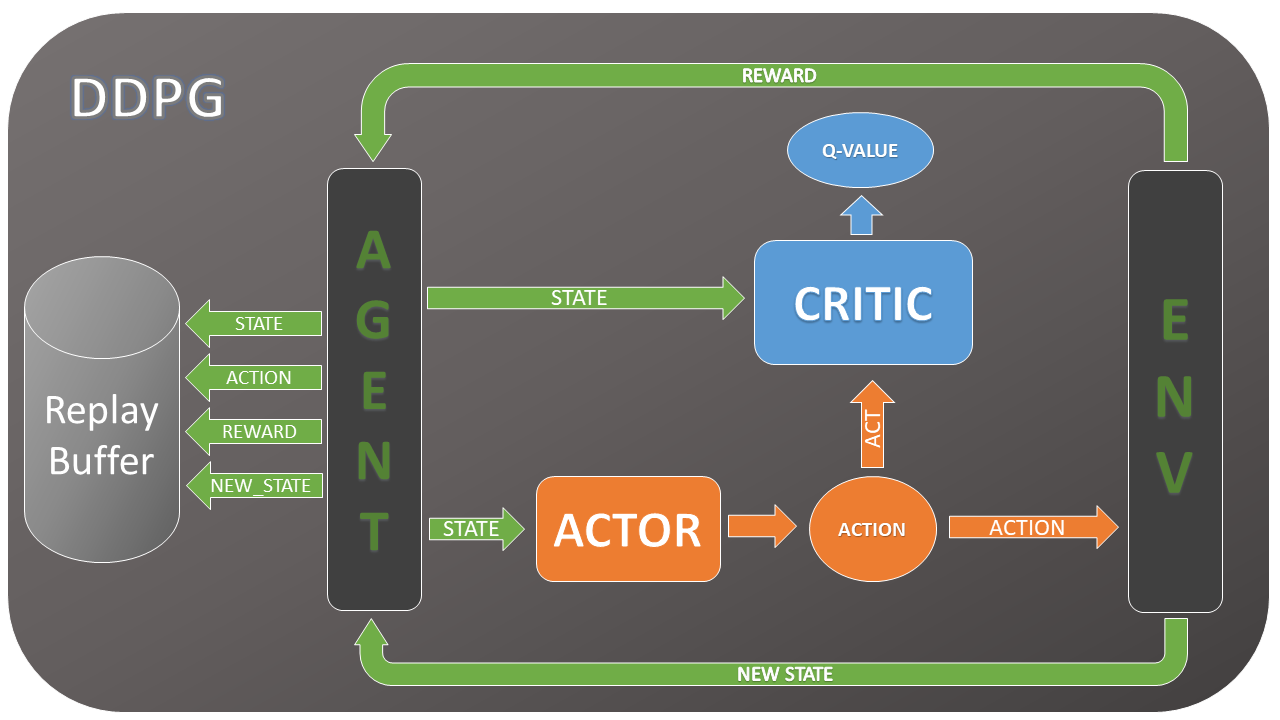
\includegraphics[width=1.\textwidth, height=.36\textheight]{pictures/ddpg_schema}
\caption{ A visual representation of the DDPG architecture. The Q-values is used only at training time.}
\end{figure}



\begin{algorithm}
	\caption{Deep Deterministic Policy Gradient}
	\label{algo:DDPG}
	\begin{algorithmic}[]
		\State Input: initial policy parameters $\theta$, Q-function parameters $\phi$, empty replay buffer {D}. 
		\State Set target parameters equal to main parameters $\theta_{targ} \leftarrow \theta $, $\phi_{targ} \leftarrow \phi $  
         \For{episode=1,M}
          
			\State Observe state s and select action $a=\operatorname{clip}\left(\mu_{\theta}(s)+\epsilon, a_{L o w}, a_{H i g h}\right),$ where $\epsilon \sim \mathcal{N}$
            \State Execute $a$ in the environment
            \State Observe next state {s'},reward {r}, and done signal {d} to indicate whether {s'} is terminal 
            \State Store (s,a,r,s',d) in replay buffer D
            \State \textbf{If} s' is terminal state reset the environment state.
            \If{it's time to update}
            	\For{however many updates}
                	\State Randomly sample a batch of transitions, $B={(s,a,r,s',d)}$ from D
                    \State Compute targets
                    \State $y\left(r, s^{\prime}, d\right)=r+\gamma(1-d) Q_{\phi_{\text {targ }}}\left(s^{\prime}, \mu_{\theta_{\text {targ }}}\left(s^{\prime}\right)\right)$
                    \State Update Q-function by one step of gradient descent using
                     \State $\nabla_{\phi} \frac{1}{|B|} \sum_{\left(s, a, r, s^{\prime}, d\right) \in B}\left(Q_{\phi}(s, a)-y\left(r, s^{\prime}, d\right)\right)^{2}$
                    \State update policy by one step of gradient ascent using:
                    \State $\nabla_{\theta} \frac{1}{|B|} \sum_{s \in B} Q_{\phi}\left(s, \mu_{\theta}(s)\right)$
                    \State Update target networks with
                    \State $\phi_{\mathrm{targ}} \leftarrow \rho \phi_{\mathrm{targ}}+(1-\rho) \phi$
					\State $\theta_{\mathrm{targ}} \leftarrow \rho \theta_{\mathrm{targ}}+(1-\rho) \theta$
                    	
                \EndFor
            \EndIf       
      \EndFor                         
	\end{algorithmic}
\end{algorithm}



